\section{Anhang}

\subsection{Vorbereitung der Python-Programme}

Führen Sie folgende Schritte durch, sofern die genannten Ordner und Dateien nicht bereits vorhanden sind:\\

\schritt{1}{Legen Sie einen Projektordner an}{

  Legen Sie auf dem Desktop des Raspberry Pi einen neuen Ordner an und nennen Sie ihn \emph{Malroboter}.\\

}

\schritt{2}{Erstellen Sie zwei neue Dateien}{

  Erstellen Sie im Ordner Malroboter die folgenden Dateien:
  \begin{itemize}
  \item \emph{motorsteuerung.py}: Diese Datei dient der Übersetzung der bestehenden Funktionen und der Definitionen innerhalb des Projektes und wird i.d.R. nicht von den Kursteilnehmern verwendet.
  \item \emph{kurs.py}: Diese Datei soll dann von den Kursteilnehmern programmiert werden, hier wird z.B. die Geschwindigkeit der Motoren eingestellt.
  \end{itemize}


}

\vspace{\baselineskip}

\schritt{3}{Fügen Sie das Steuerungsprogramm ein}{

 Fügen Sie den folgenden Programmtext in die Datei \emph{motorsteuerung.py} ein:\\
  \indent \hinweis Sie finden die Programmdateien auch \href{https://www.github.com/latenighticecream/malroboter/Malroboter}{hier}\footnote[2]{https://www.github.com/latenighticecream/malroboter/Malroboter}.\\

}

\emph{motorsteuerung.py}\\
\lstinputlisting{Malroboter/motorsteuerung.py}
\vspace{\baselineskip}

\schritt{4}{Binden Sie das Steuerungsprogramm ein}{
Öffnen Sie die Datei \emph{kurs.py} und fügen sie den folgenden Programmtext ein:
\lstinputlisting{Malroboter/kurs.py}
}

Dies bindet die Definition innerhalb der Datei motorsteuerung.py in die Kursdatei ein, sodass sie dort verwendet werden können.

\subsection{Anbringen der Motorkabel}
Sollten die Motoren noch keine Kabel angebracht haben, muss das natürlich noch passieren. Dazu benötigen Sie pro Motor zwei einfache Kabel und eine Möglichkeit, deren Isolierung zu entfernen.

\schritt{1}{Kabel abisolieren}{
  Isolieren Sie die Kabel auf etwa 0.5 bis 1 cm ab.\\
}

\schritt{2}{Kabel am Motor anbringen}{
  Stecken Sie die Kabel jeweils durch eine der Ösen an den Motorkontakten und knicken diese um.\\
}

\schritt{3}{(Optional) Kabel verlöten}{
  Löten Sie die Kabel an den Motorkontakten an. Dieser Schritt ist optional, bietet jedoch einen stabileren und zuverlässigeren Kontakt.\\
}

\begin{center}
  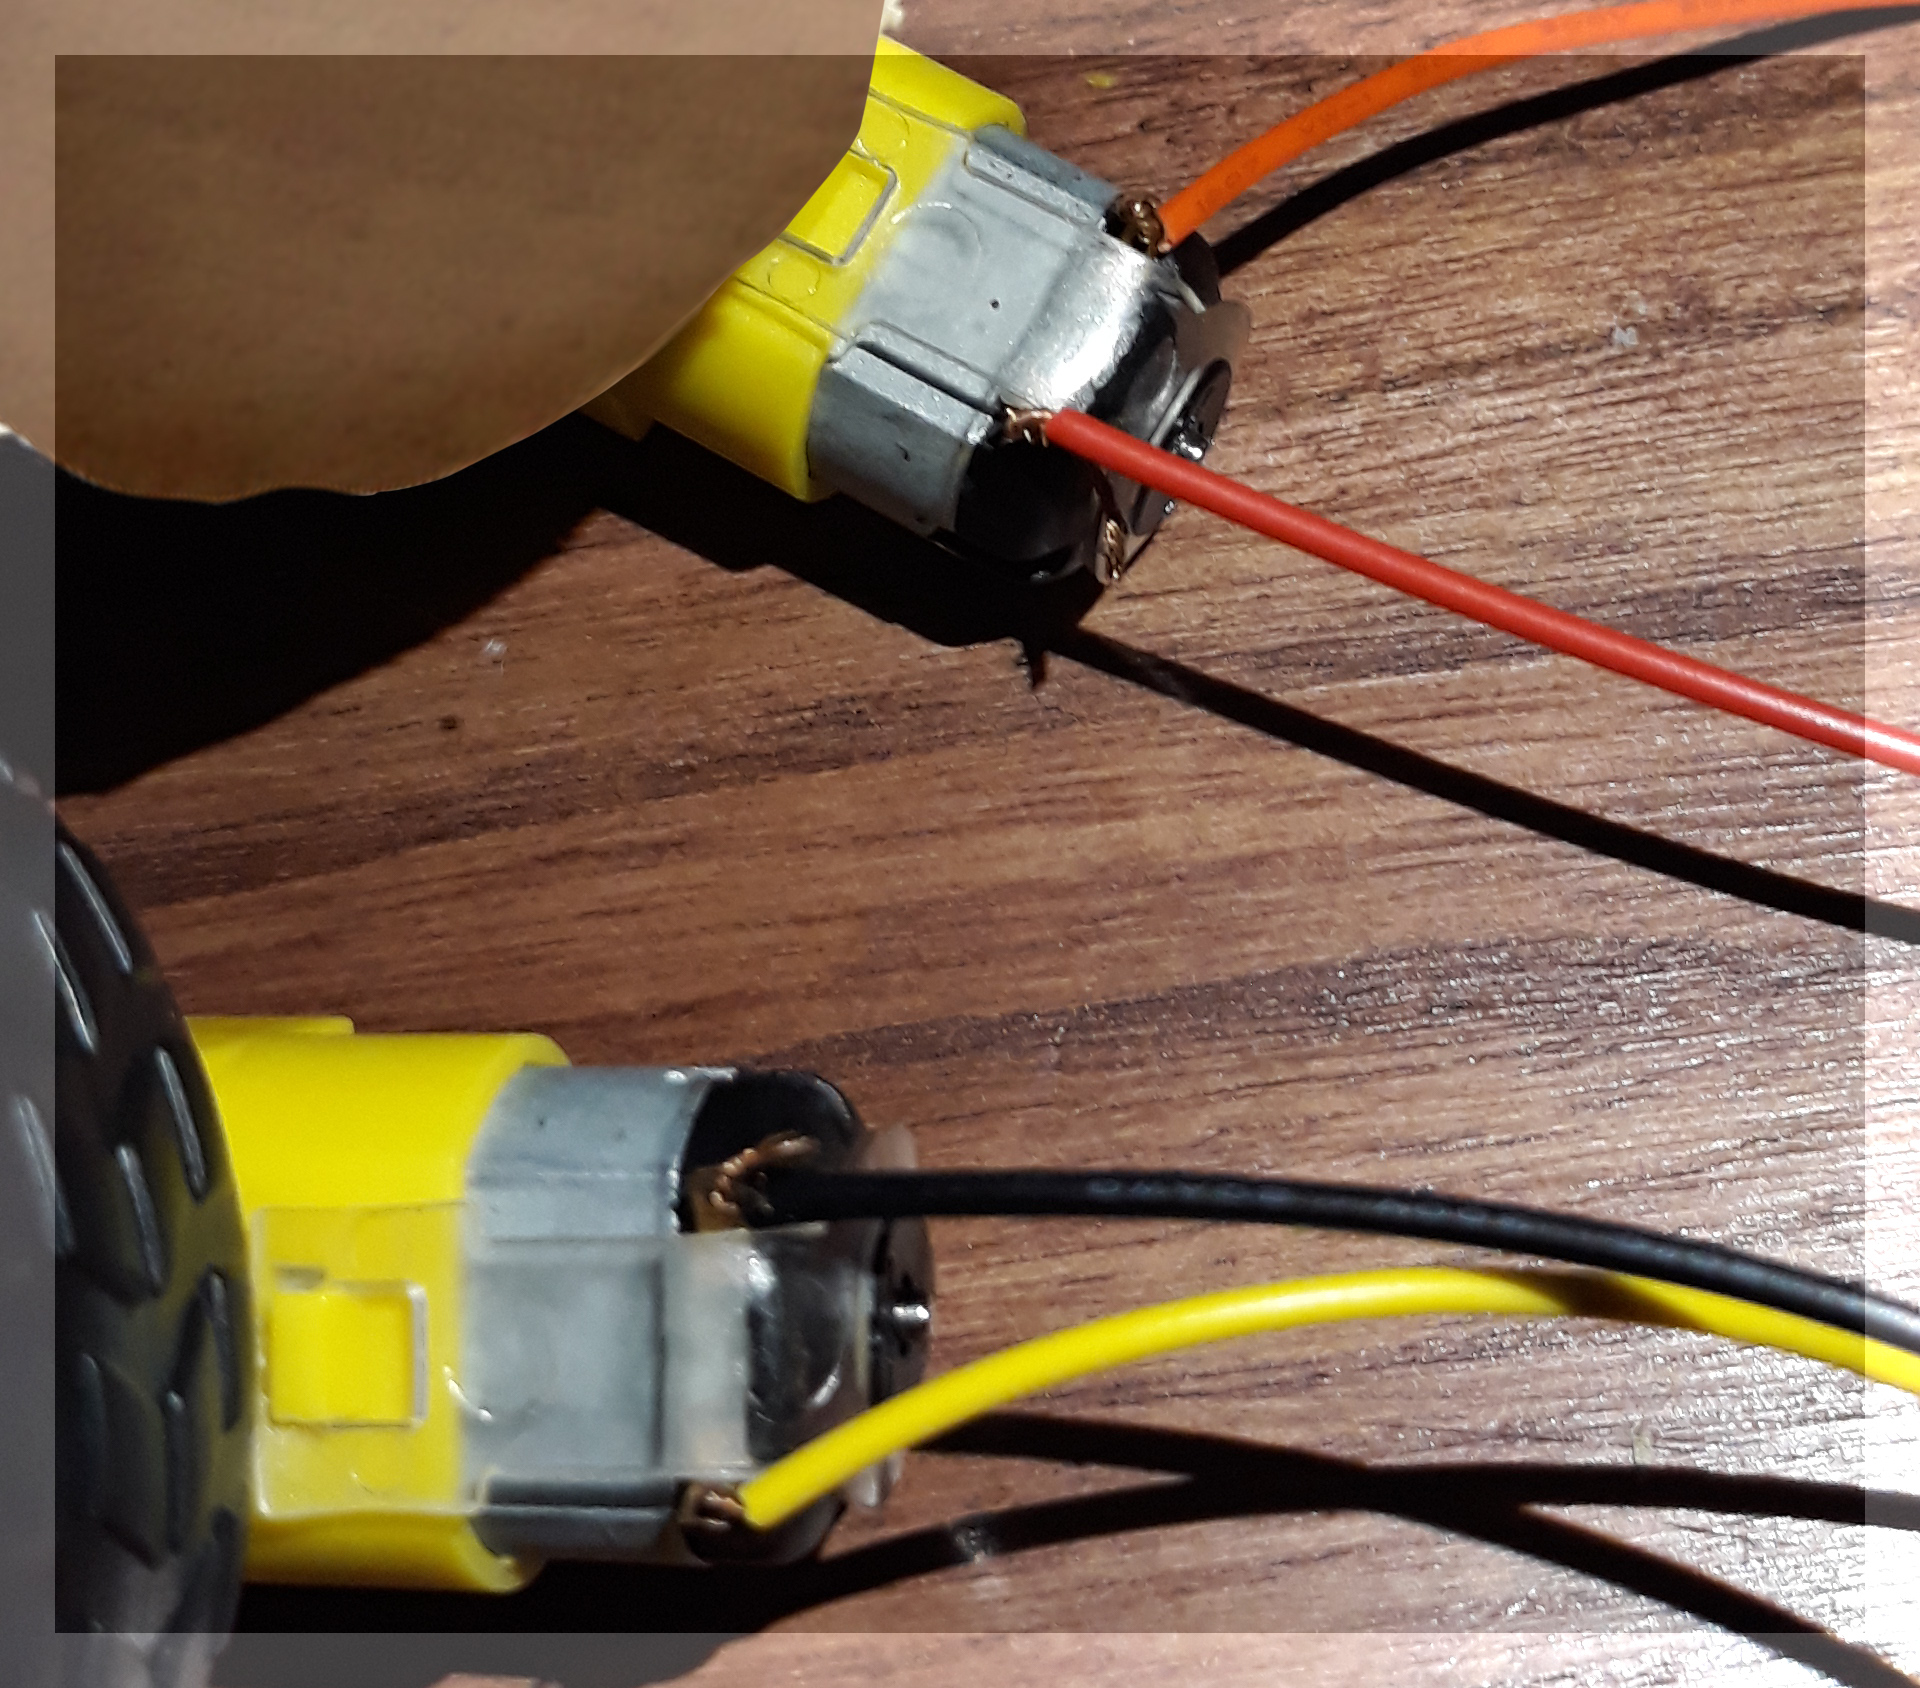
\includegraphics[width=\textwidth]{motor_close.jpg}
\end{center}
